\documentclass{beamer}

\usetheme{Padova}
%\setbeamercovered{transparent}
%\usefonttheme{metropolis}

\newcommand{\backupbegin}{
	\newcounter{framenumberappendix}
	\setcounter{framenumberappendix}{\value{framenumber}}
}
\newcommand{\backupend}{
	\addtocounter{framenumberappendix}{-\value{framenumber}}
	\addtocounter{framenumber}{\value{framenumberappendix}} 
}

\title{Towards Explainability in Knowledge Enhanced Neural Networks}
\subtitle{Data Science Master Thesis}
\author{Riccardo Mazzieri}
\date{September 21, 2021}


\begin{document}

	\maketitle

	\begin{frame}{Outline}
		\tableofcontents
	\end{frame}


	\section{Introduction}

	\begin{frame}{Introduction}
		Deep NNs have several flaws. For example:
		\begin{itemize}
%			\pause
			\item They are \textbf{data hungry}:
			\begin{itemize}
				\item With few data, learning is not possible, even for simple logical reasoning tasks;
				\item This motivates \textbf{Neural Symbolic Integration (NeSy)}.
%				research field that focuses on the integration of logic inside neural networks
			\end{itemize}
%			\pause6
			\item They are \textbf{black boxes}:
			\begin{itemize}
				\item Decisions are not explainable, might lead to lack of trust in AI applications;
				\item This motivates the research field of \textbf{Explainable AI (XAI)}.
			\end{itemize}
		\end{itemize}
	\end{frame}


	\section{KENN}

	\begin{frame}{Knowledge Enhanced Neural Networks}
		KENN consists in a residual layer designed to improve the predictions of a base NN, by using logical prior knowledge, consisting in a set of FOL formulas $\mathcal{K}$.
		\begin{figure}
			\centering
			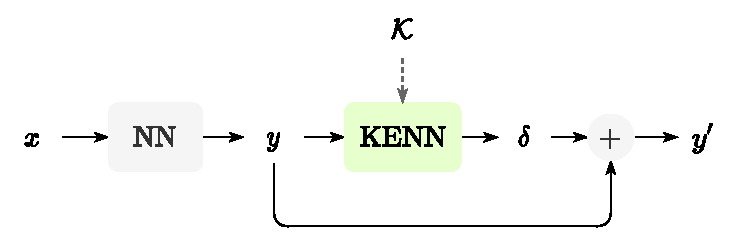
\includegraphics[width=0.95\linewidth]{images/kenn_intuition.pdf}
			
		\end{figure}
	\end{frame}

\begin{frame}{Basic Terminology}
	\begin{definition}[The Language]
		Our language will be a function-free first order language $\mathcal{L}$, defined by:
		\begin{itemize}
			\item A set of \textbf{constants}: $\mathcal{C}=\{a_1,\dots,a_{|\mathcal{C}|}\}$;
			\item A set of \textbf{predicates}: $\mathcal{P}=\{P_1,\dots,P_{|\mathcal{P}|}\}$;
		\end{itemize}
	\end{definition}

	
	\begin{definition}[Clause]
		A clause $c$ is a formula expressed a disjunction of literals:
		\begin{equation*}
		c:=\bigvee_{i=1}^{k} l_{i}, \quad l_{i} \neq l_{j} \quad \forall i \neq j
		\end{equation*}
	\end{definition}
\end{frame}

%\begin{frame}{Example}
%	Given two predicates $\text{Smoke}$ and $\text{Friends}$, an example of formula is:
%	$$c: \forall x,\forall y \quad \operatorname{Smoke}(x) \wedge \operatorname{Friends}(x,y) \Rightarrow \operatorname{Smoke}(y).$$
%	
%	\pause
%	
%	Inside KENN, formulas are represented as a disjunction of literals, and are evaluated on constants.
%	For example, given two constants $a_1$ and $a_2$, the following clause:
%	
%	$$\neg \operatorname{Smoke}(a_1) \vee \neg \operatorname{Friends}(a_1,a_2) \vee \operatorname{Smoke}(a_2). $$
%	is called the \textbf{grounding} of $c$.
%\end{frame}

\begin{frame}{Language Semantic}
			\begin{figure}
		\centering
		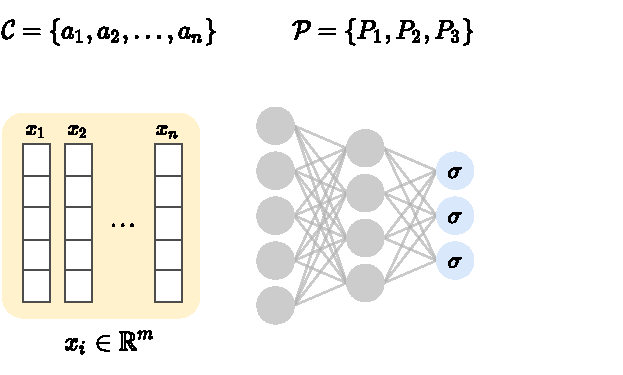
\includegraphics[width=\linewidth]{images/interpretation_intuition0.pdf}
	\end{figure}
	
\end{frame}
\begin{frame}{Language Semantic}
	\begin{figure}
		\centering
		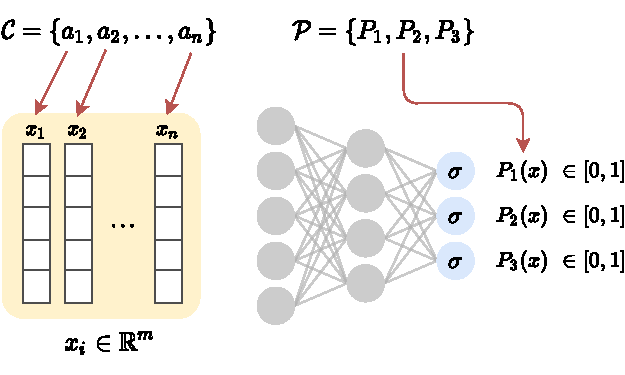
\includegraphics[width=\linewidth]{images/interpretation_intuition1.pdf}
	\end{figure}
\end{frame}

\begin{frame}{Language Semantic}
	 Note that truth values can be any real number in $[0,1]$\\ $  \Rightarrow$ We will follow the rules of \textbf{Fuzzy Logic}, an extension of Boolean Logic. Specifically, in Fuzzy logic:
	\begin{itemize}
		\pause
		\item Truth value of a negated predicate is simply $\mathcal{I}(\neg A(x)) = 1 - \mathcal{I}(A(x))$
		\pause
		\item Truth value of a disjunction of literals is computed by means of a \textbf{$t$-conorm} function;
		\pause
		\item KENN uses the Gödel $t$-conorm, which is defined as:
		\begin{equation*}
		\perp_{\text{max}}(t) = \underset{i=1,\dots,m}{\operatorname{max}} t_i, \quad \forall t\in [0,1]^m.
		\end{equation*}
	\end{itemize}	
\end{frame}

%\begin{frame}{Example}
%	\begin{exampleblock}{Example: truth value of a clause}
%		Suppose that, given the constant term $a$, the truth value of $\text{Dog}(a)$ is $0.8$, the one for $\text{Animal}(a)$ is $0.5$ and the one for $\text{Human}(a)$ is $0.3$. Then, the truth value of the grounded clause
%		$$c: \neg \text{Dog}(a) \vee \text{Animal}(a)$$  
%		will be:
%		\begin{equation*}
%		\perp_{\text{max}}(1-0.8,0.5) = \underset{i=1,\dots,m}{\operatorname{max}}(0.2,0.5) = 0.5.
%		\end{equation*}
%		Note how $\text{Human}(a)$ is not considered for this computation, since it does not appear in $c$.
%		
%	\end{exampleblock}
%\end{frame}

\begin{frame}{Example: truth value of a clause}
	\begin{figure}
		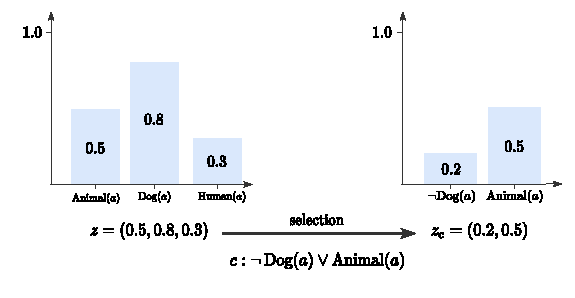
\includegraphics[width=\linewidth]{images/example_clause_boosting0.pdf}
	\end{figure}
\end{frame}

\begin{frame}{Example: truth value of a clause}
	\begin{figure}
		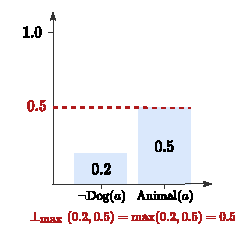
\includegraphics[width=0.6\linewidth]{images/tvalues_literals.pdf}
	\end{figure}
\end{frame}

\begin{frame}{Increasing satisfaction of a single clause}
	Given the vector of predictions of the NN $y$ and given $c\in \mathcal{K}$, KENN computes a vector of changes $\delta^c$, such that the final vector of predictions $y' = y +\delta^c$:
	\begin{itemize}
		\item Improves the truth value of $c$,
		\item Keeps the quantity $\|y'-y \|_2$ minimal.
	\end{itemize}
\end{frame}

\begin{frame}{Increasing satisfaction of a single clause}
	\begin{figure}
		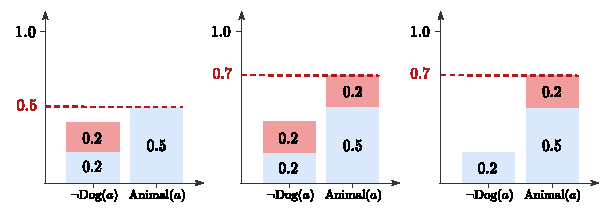
\includegraphics[width=\linewidth]{images/boost_options.pdf}
	\end{figure}
\pause
%	Given the vector of truth values of the literals $z_c$, this delta is coputed as follows:
	\begin{equation*}
	\delta_{s}^{w_{c}}\left(z_{c}\right)=w_{c} \cdot \operatorname{softmax}\left(z_{c}\right)
%	\label{eq:clause_enhancement}
	\end{equation*}
\end{frame}


\begin{frame}{Boosting Preactivations}
	In practice, inside KENN the delta vectors are applied to the \textbf{preactivations} from the NN:
	\begin{equation*}
	y'=\sigma(z + \delta^c).
	\end{equation*}
	\pause
	Then, in order to increase the satisfaction of the entire knowledge, all the deltas are aggregated by being summed together. The final prediction will be:
	\begin{equation*}
	y^{\prime}=\sigma\left(z+\sum_{c \in \mathcal{K}} \delta^{c}\right).
	\end{equation*}
\end{frame}


%\begin{frame}{KENN for relational data}
%	\begin{itemize}
%		\item KENN can deal also with binary clauses, meaning clauses that contain binary predicates and express \textbf{relations} between objects;
%		\item This is done by considering unary and binary clauses separately, and computing the final prediction as follows:
%	\end{itemize}
%	 
%	\begin{equation*}
%	y^{\prime}=\sigma\left(z+\sum_{c \in \mathcal{K}_{U}} \delta^{c}+\sum_{c \in \mathcal{K}_{B}} \delta^{c}\right)
%	\end{equation*}
%\end{frame}
%
%\begin{frame}{Relational data representation}
%		\begin{figure}[h]
%		\centering
%		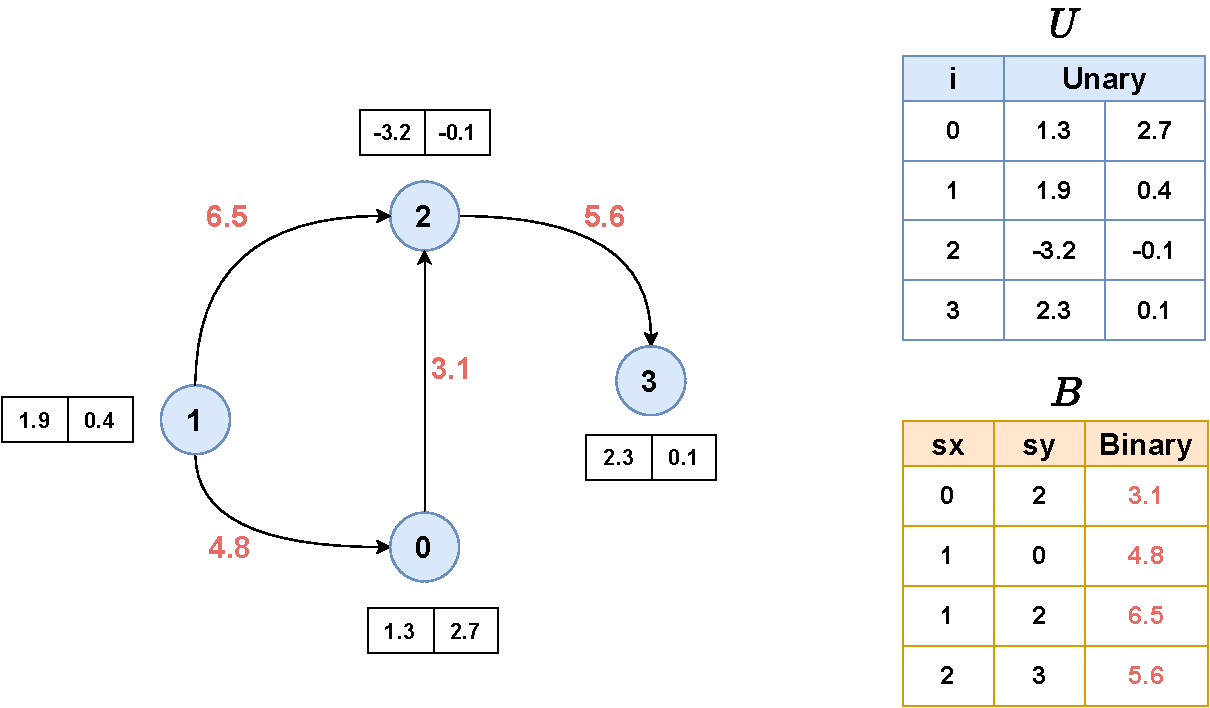
\includegraphics[width=0.8\linewidth]{images/kenn_relational_representation2.pdf}
%	\end{figure}
%\begin{equation*}
%\left\{\begin{array}{l}
%y_{u}^{\prime}=\sigma(U+\delta U) \\
%y_{b}^{\prime}=\sigma(B+\delta B)
%\end{array}\right.
%\end{equation*}
%
%\end{frame}
%
%\begin{frame}{Relational data representation}
%	\begin{figure}[h]
%		\centering
%		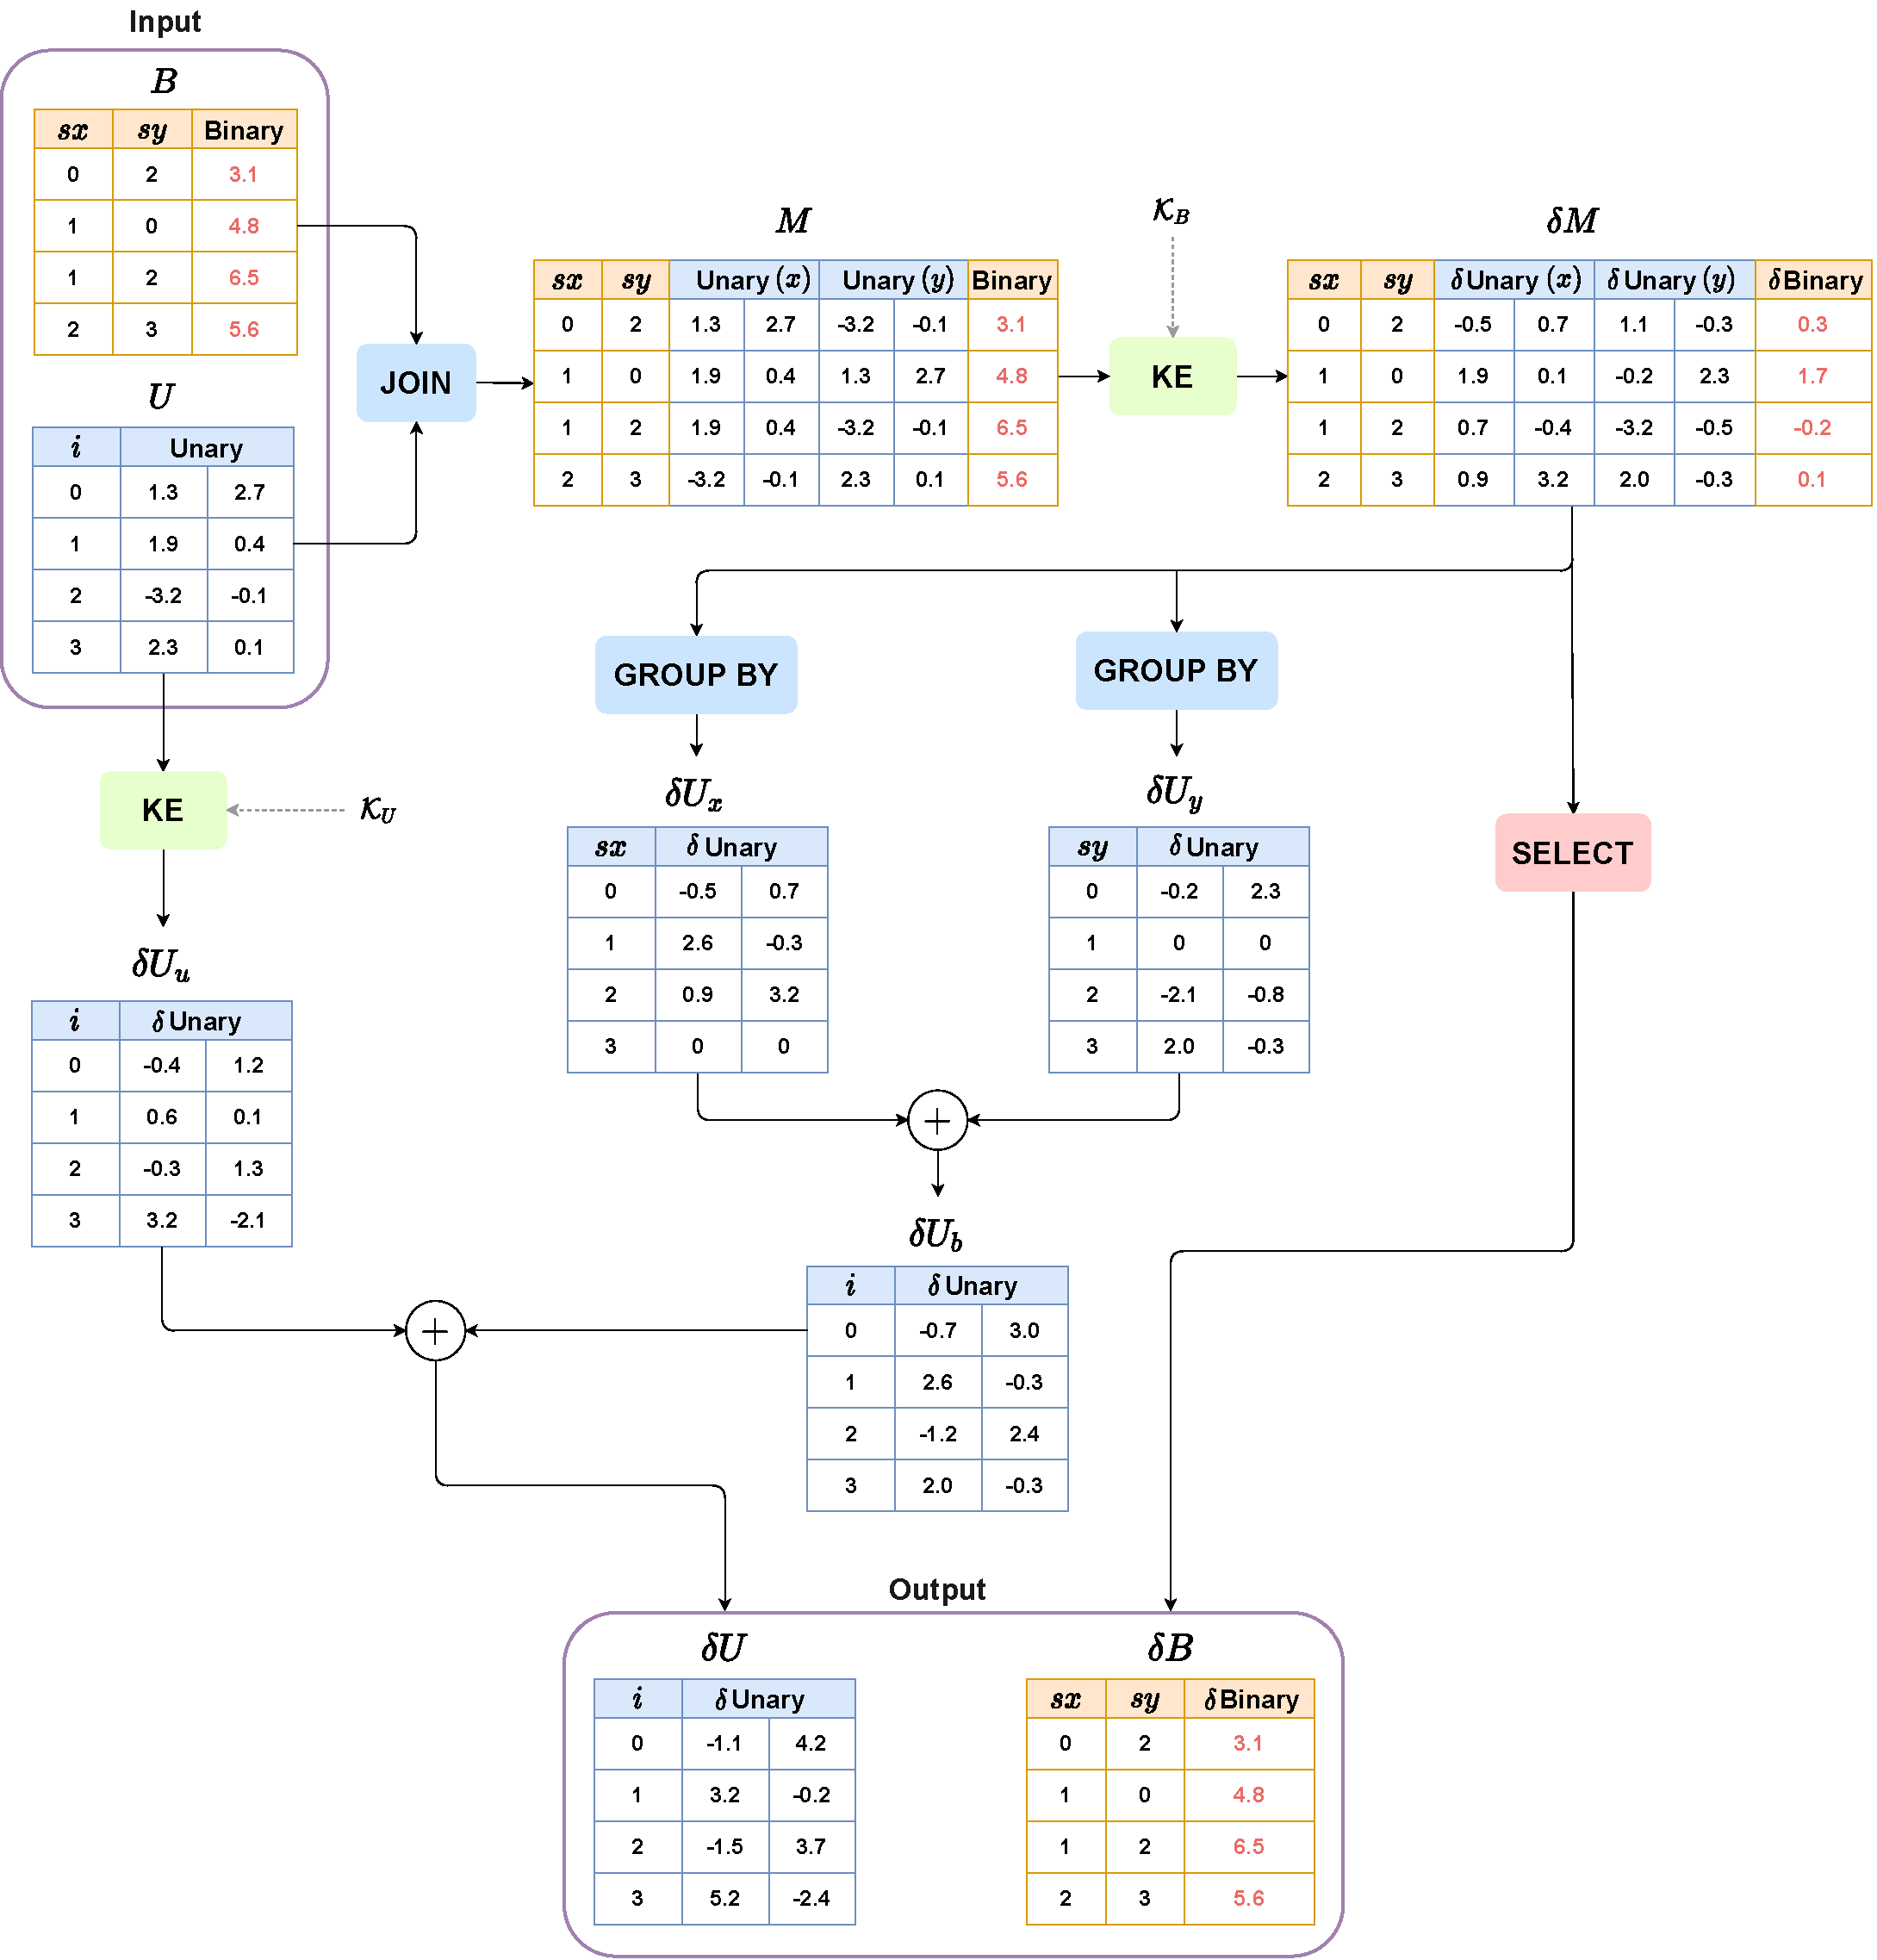
\includegraphics[width=0.6\linewidth]{images/kenn_relational_global_chart.pdf}
%	\end{figure}
%\end{frame}

\section{Experiments on Collective Classification}

\begin{frame}{Citeseer Experiments}
	\begin{itemize}
		\item We tested KENN on a Collective Classification task;
		\item The \textbf{Citeseer Dataset} was used: citation network with $4732$ citations (edges) between $3312$ papers (nodes);
		\item The task is to predict the topic of each paper.
	\end{itemize}

\begin{figure}
	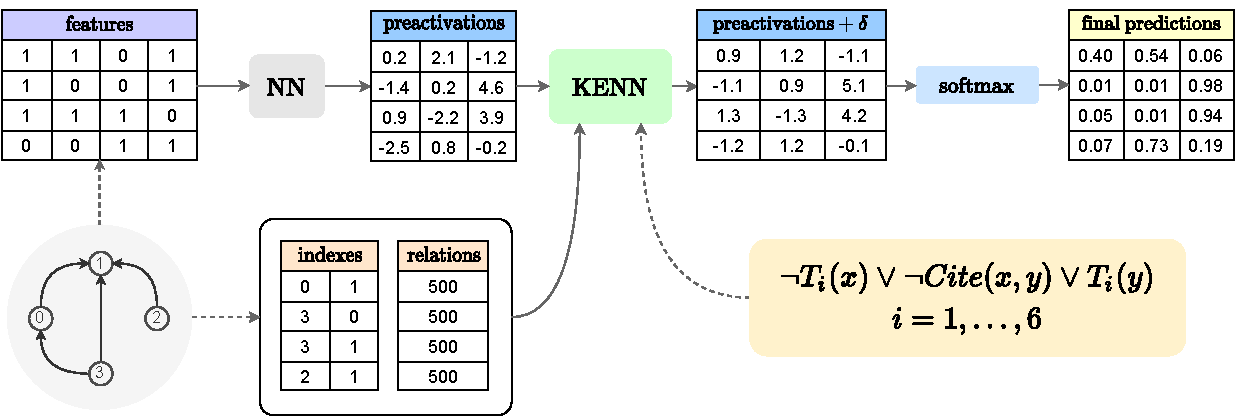
\includegraphics[width=\linewidth]{images/citeseer_setup_pres.pdf}
\end{figure}
\end{frame}

\begin{frame}{Learning Paradigms}
	\begin{figure}
		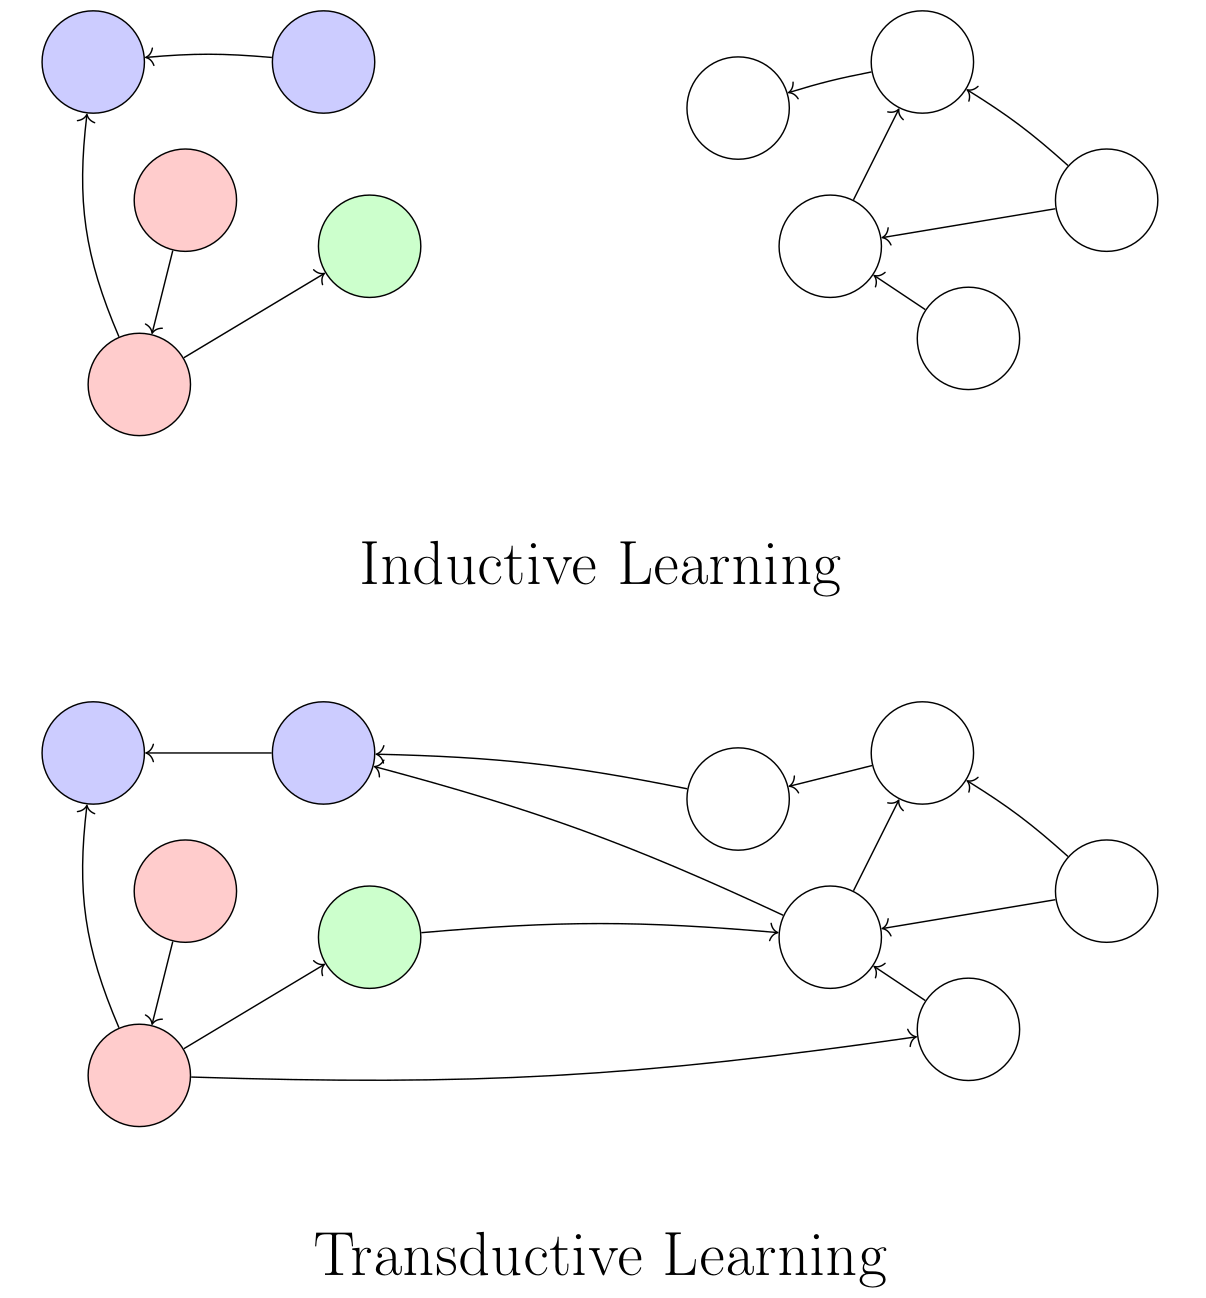
\includegraphics[width=0.58\linewidth]{images/ind_vs_trans.png}
	\end{figure}
\end{frame}


\begin{frame}{Results Inductive Paradigm}
	\begin{figure}
		\centering
		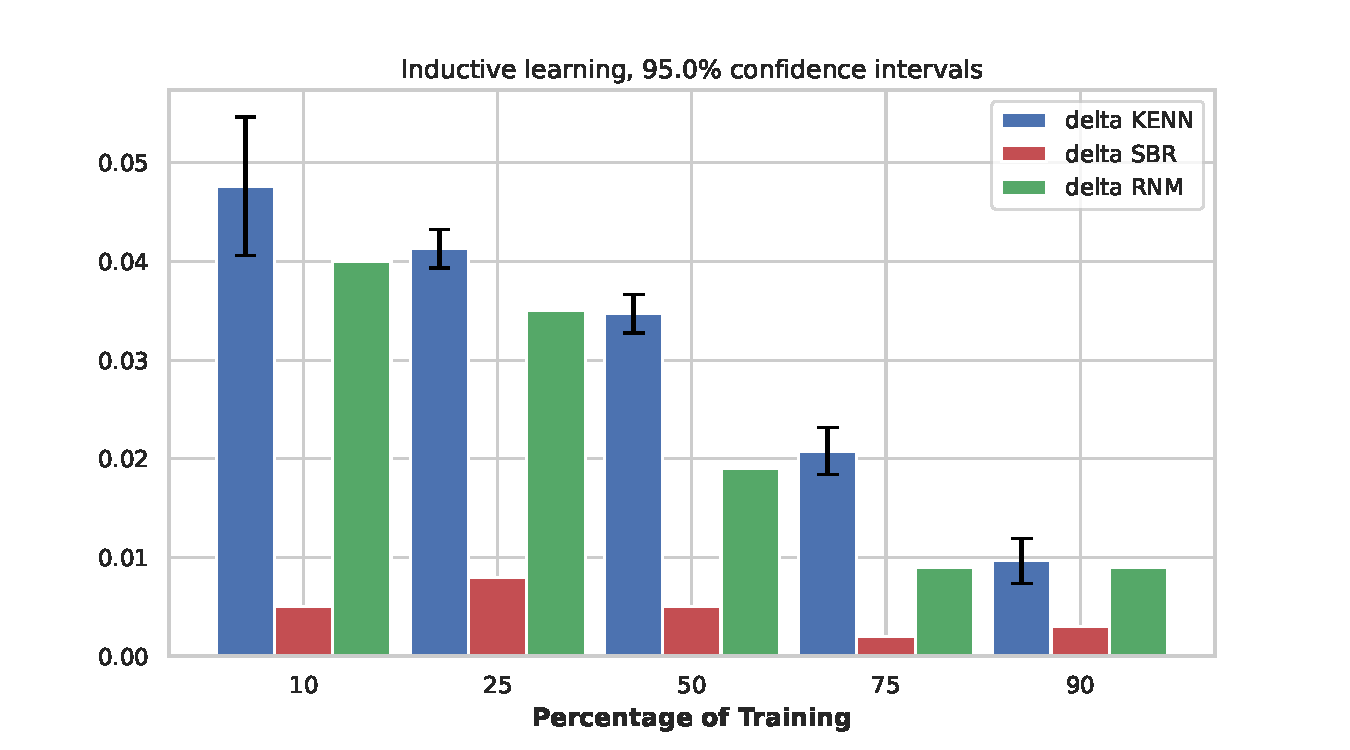
\includegraphics[width=\linewidth]{images/deltas_inductive.pdf}
		\caption{Relative improvements for the Inductive Paradigm}
	\end{figure}
\end{frame}

\begin{frame}{Results Transductive Paradigm}
	\begin{figure}
		\centering
		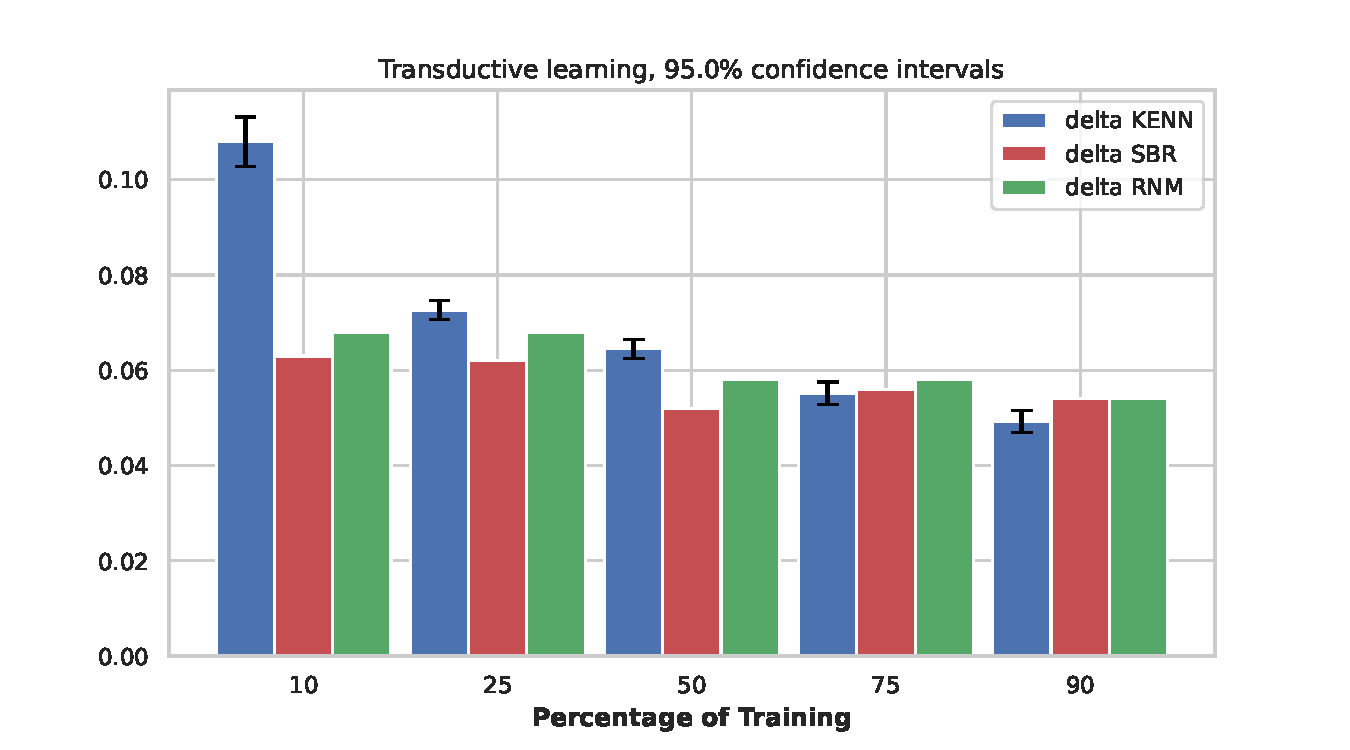
\includegraphics[width=\linewidth]{images/deltas_transductive.pdf}
		\caption{Relative improvements for the Transductive Paradigm}
	\end{figure}
\end{frame}

\section{Explainability in KENN}

\begin{frame}{Explainability}
	\begin{definition}[Explainability]
		We define explainability in the context of supervised ML
		as the \textbf{generic process by which we extract any kind of explanation from a model}. This can
		be done by exploiting the natural properties of the model (in which case, such a model can be
		called explainable), or by devising techniques to extract explanations from any model.
	\end{definition}

\end{frame}

\begin{frame}{Explainability}
	In XAI, two main paradigms for explainability are distinguished: 
	\begin{itemize}
		\item \textbf{Transparency}
		\item \textbf{Post-hoc explainability}
	\end{itemize}
	\begin{figure}
		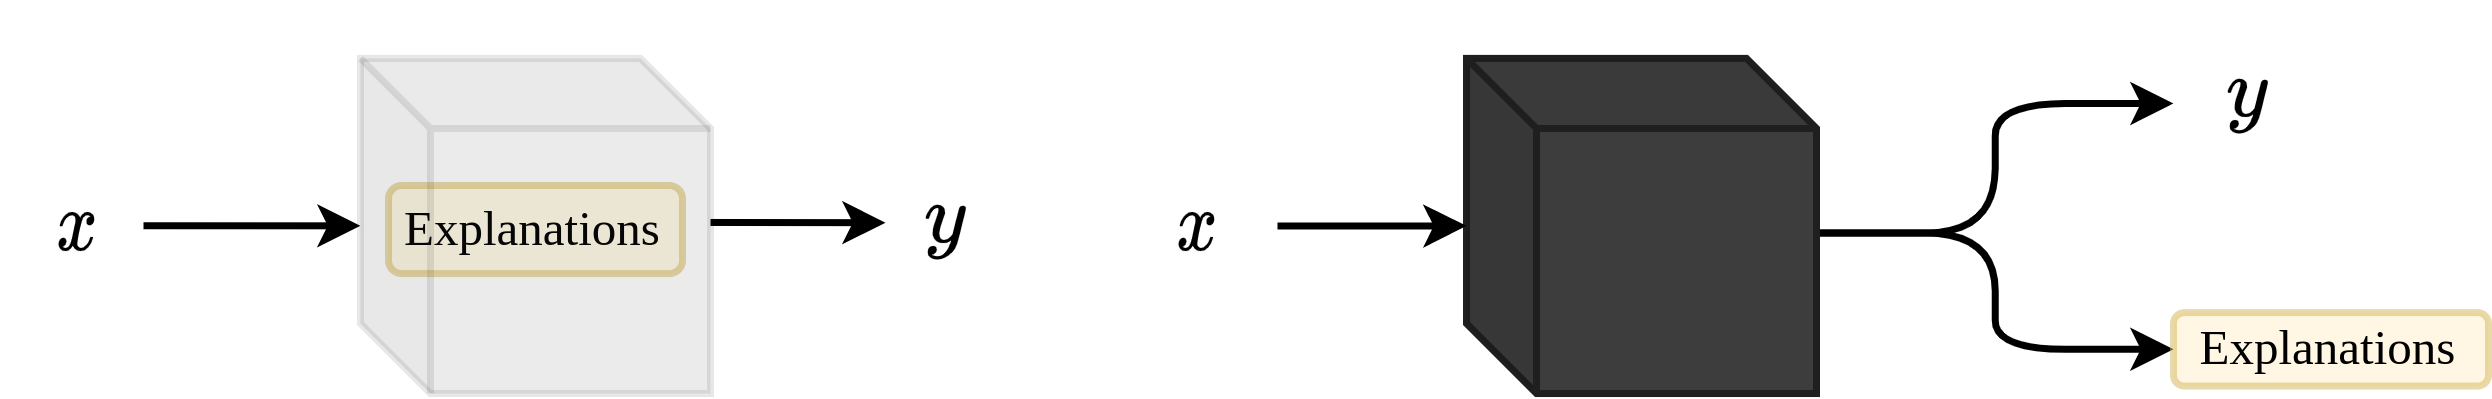
\includegraphics[width=\linewidth]{images/trasparency_vs_posthoc.png}
	\end{figure}
\end{frame}

\begin{frame}{Activation Maximization}
	\begin{figure}
		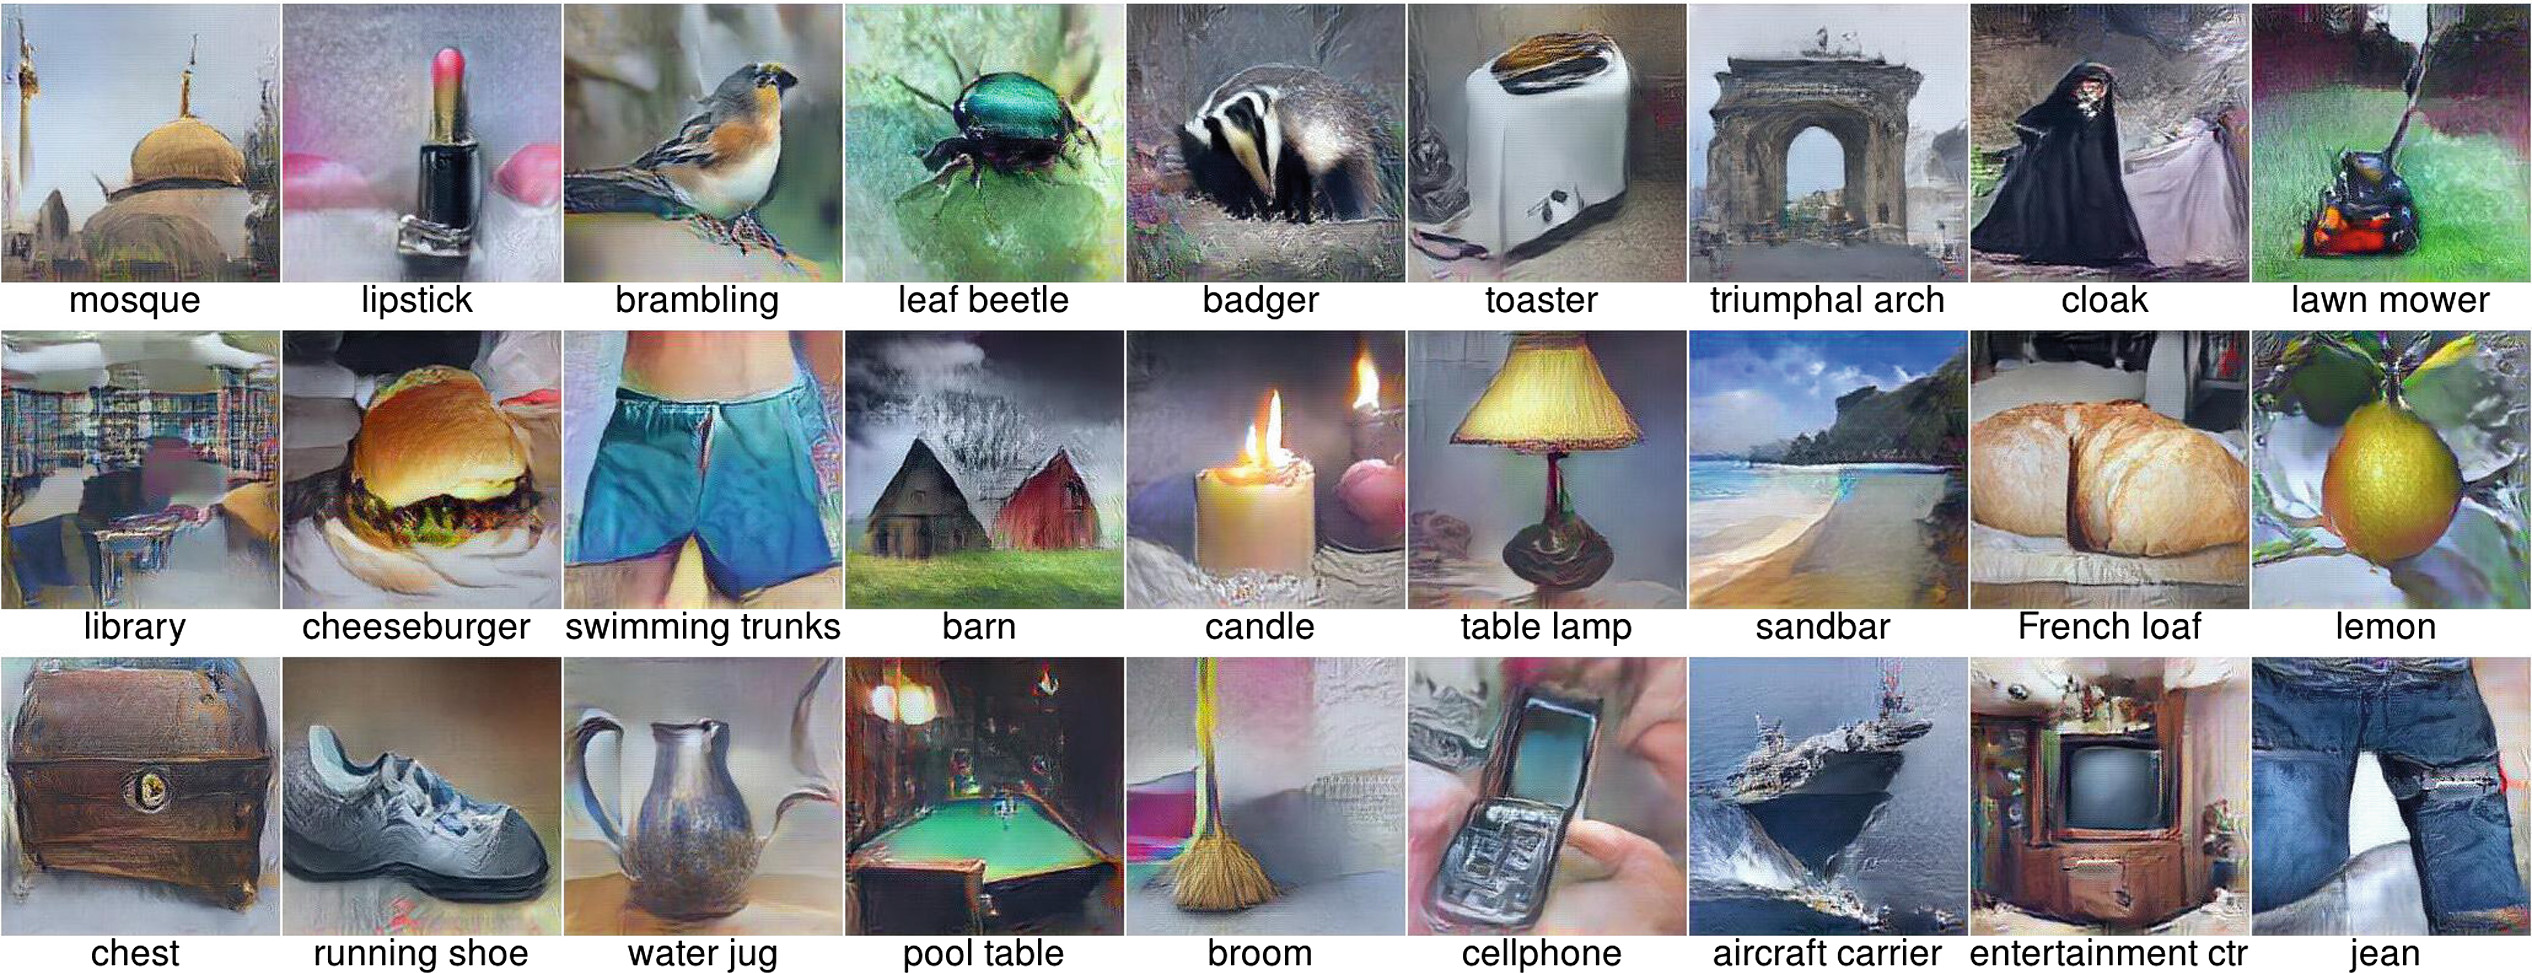
\includegraphics[width=\linewidth]{images/activation_maximization.png}
	\end{figure}
\begin{equation*}
x_{i}^{*}=\max _{x} \log p\left(\omega_{i} \mid x\right)-\lambda\|x\|^{2}
\end{equation*}
\end{frame}

\begin{frame}{Local Explanations: saliency maps}
	\begin{figure}
		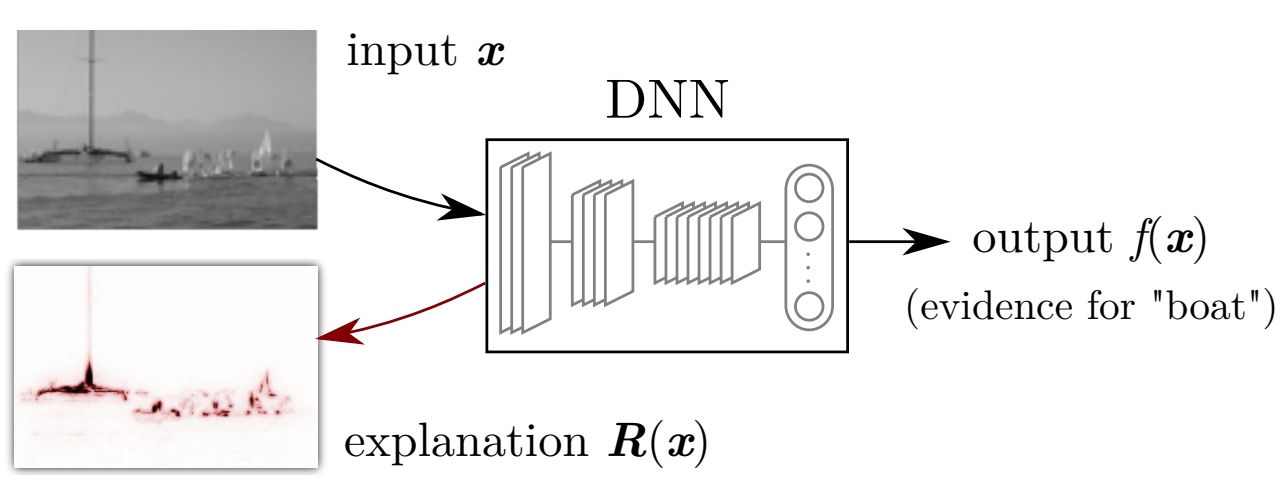
\includegraphics[width=0.8\linewidth]{images/explanation_map_nn.png}
	\end{figure}
	\begin{equation*}
	R(x)_{i}=\left(\frac{\partial f}{\partial x_{i}}\right)^{2}
	\end{equation*}
\end{frame}

\begin{frame}{Explainability in KENN}
KENN can be considered a \textbf{partially transparent} model:
\begin{itemize}
	\item A KENN layer will always be based on the prediction of a base NN, which will always be an inherently opaque model;
	\item On the contrary, everything happening inside the KENN layer is transparent;
	\item The explanations will only regard the knowledge enforcement stage.
\end{itemize}
\end{frame}

\begin{frame}{Local explanations from a single clause}
	Esempio...
\end{frame}

\begin{frame}{Assessing impact of more clauses}
	Custom score.
\end{frame}

\definecolor{unipd}{rgb}{.7,.105,.109}

\begin{frame}{}
	\centering \Large
	\textcolor{unipd}{\textbf{Thank you for your attention}}
\end{frame}

\appendix
\backupbegin

\begin{frame}{Appendix: Clause Enhancer}
	\begin{figure}
		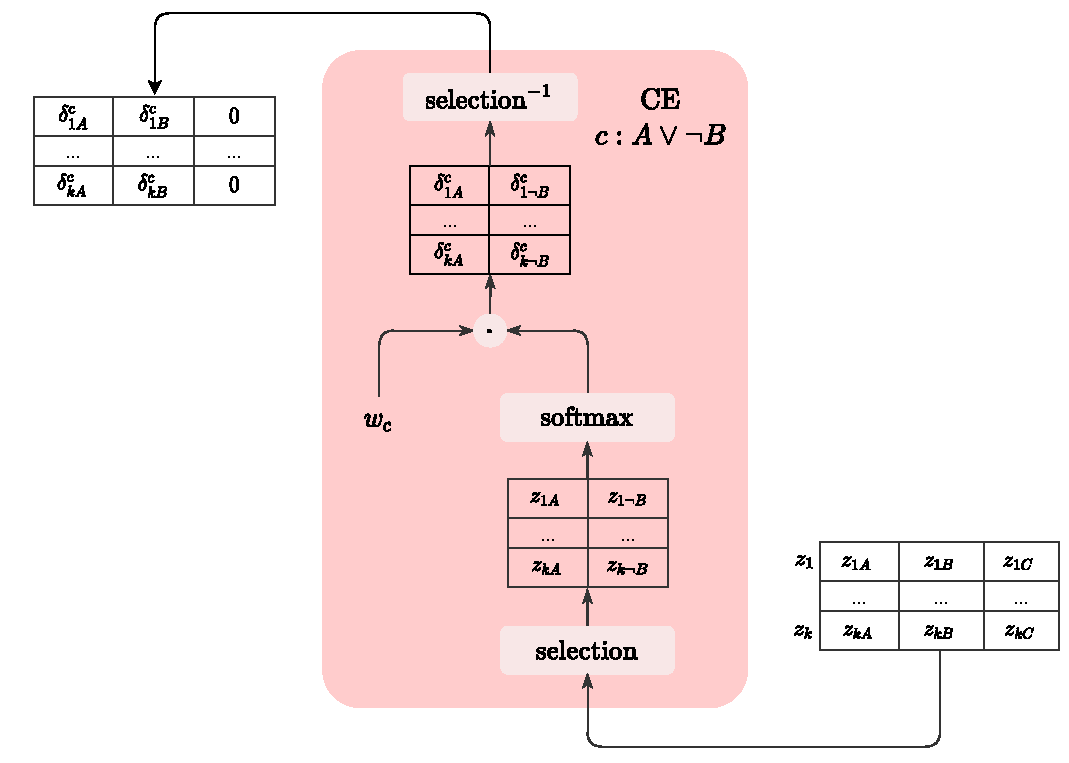
\includegraphics[width=0.9\linewidth]{images/CE_presentation.pdf}
	\end{figure}
\end{frame}

\begin{frame}{Appendix: Knowledge Enhancer}
	\begin{figure}
		\centering
		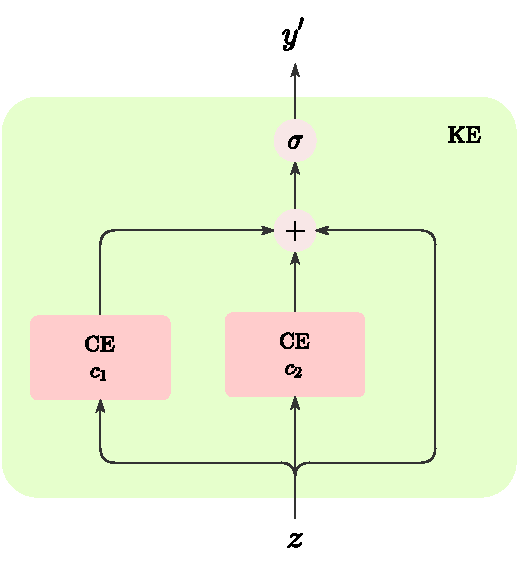
\includegraphics[width=0.55\linewidth]{images/KE.pdf}
	\end{figure}
\end{frame}

\begin{frame}{Appendix: KENN for relational data}
	\begin{figure}
		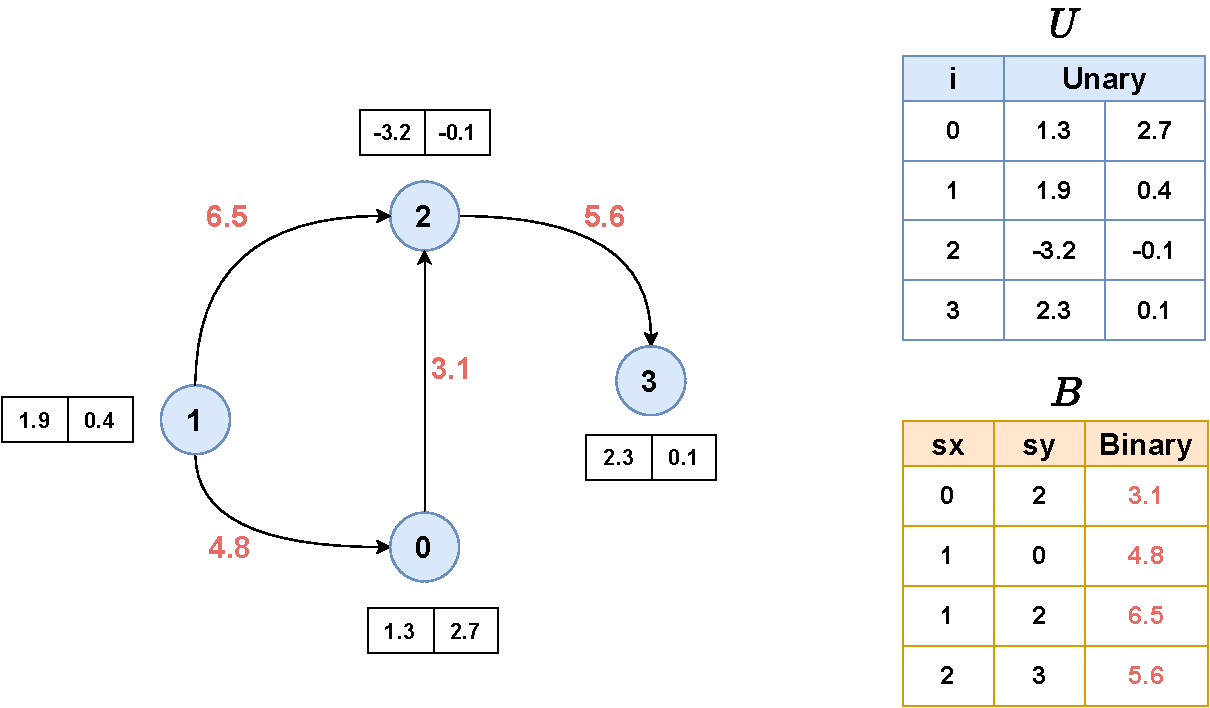
\includegraphics[width=0.9\linewidth]{images/kenn_relational_representation2.pdf}
	\end{figure}
\end{frame}

\begin{frame}{Appendix: KENN for relational data}
	\begin{figure}
		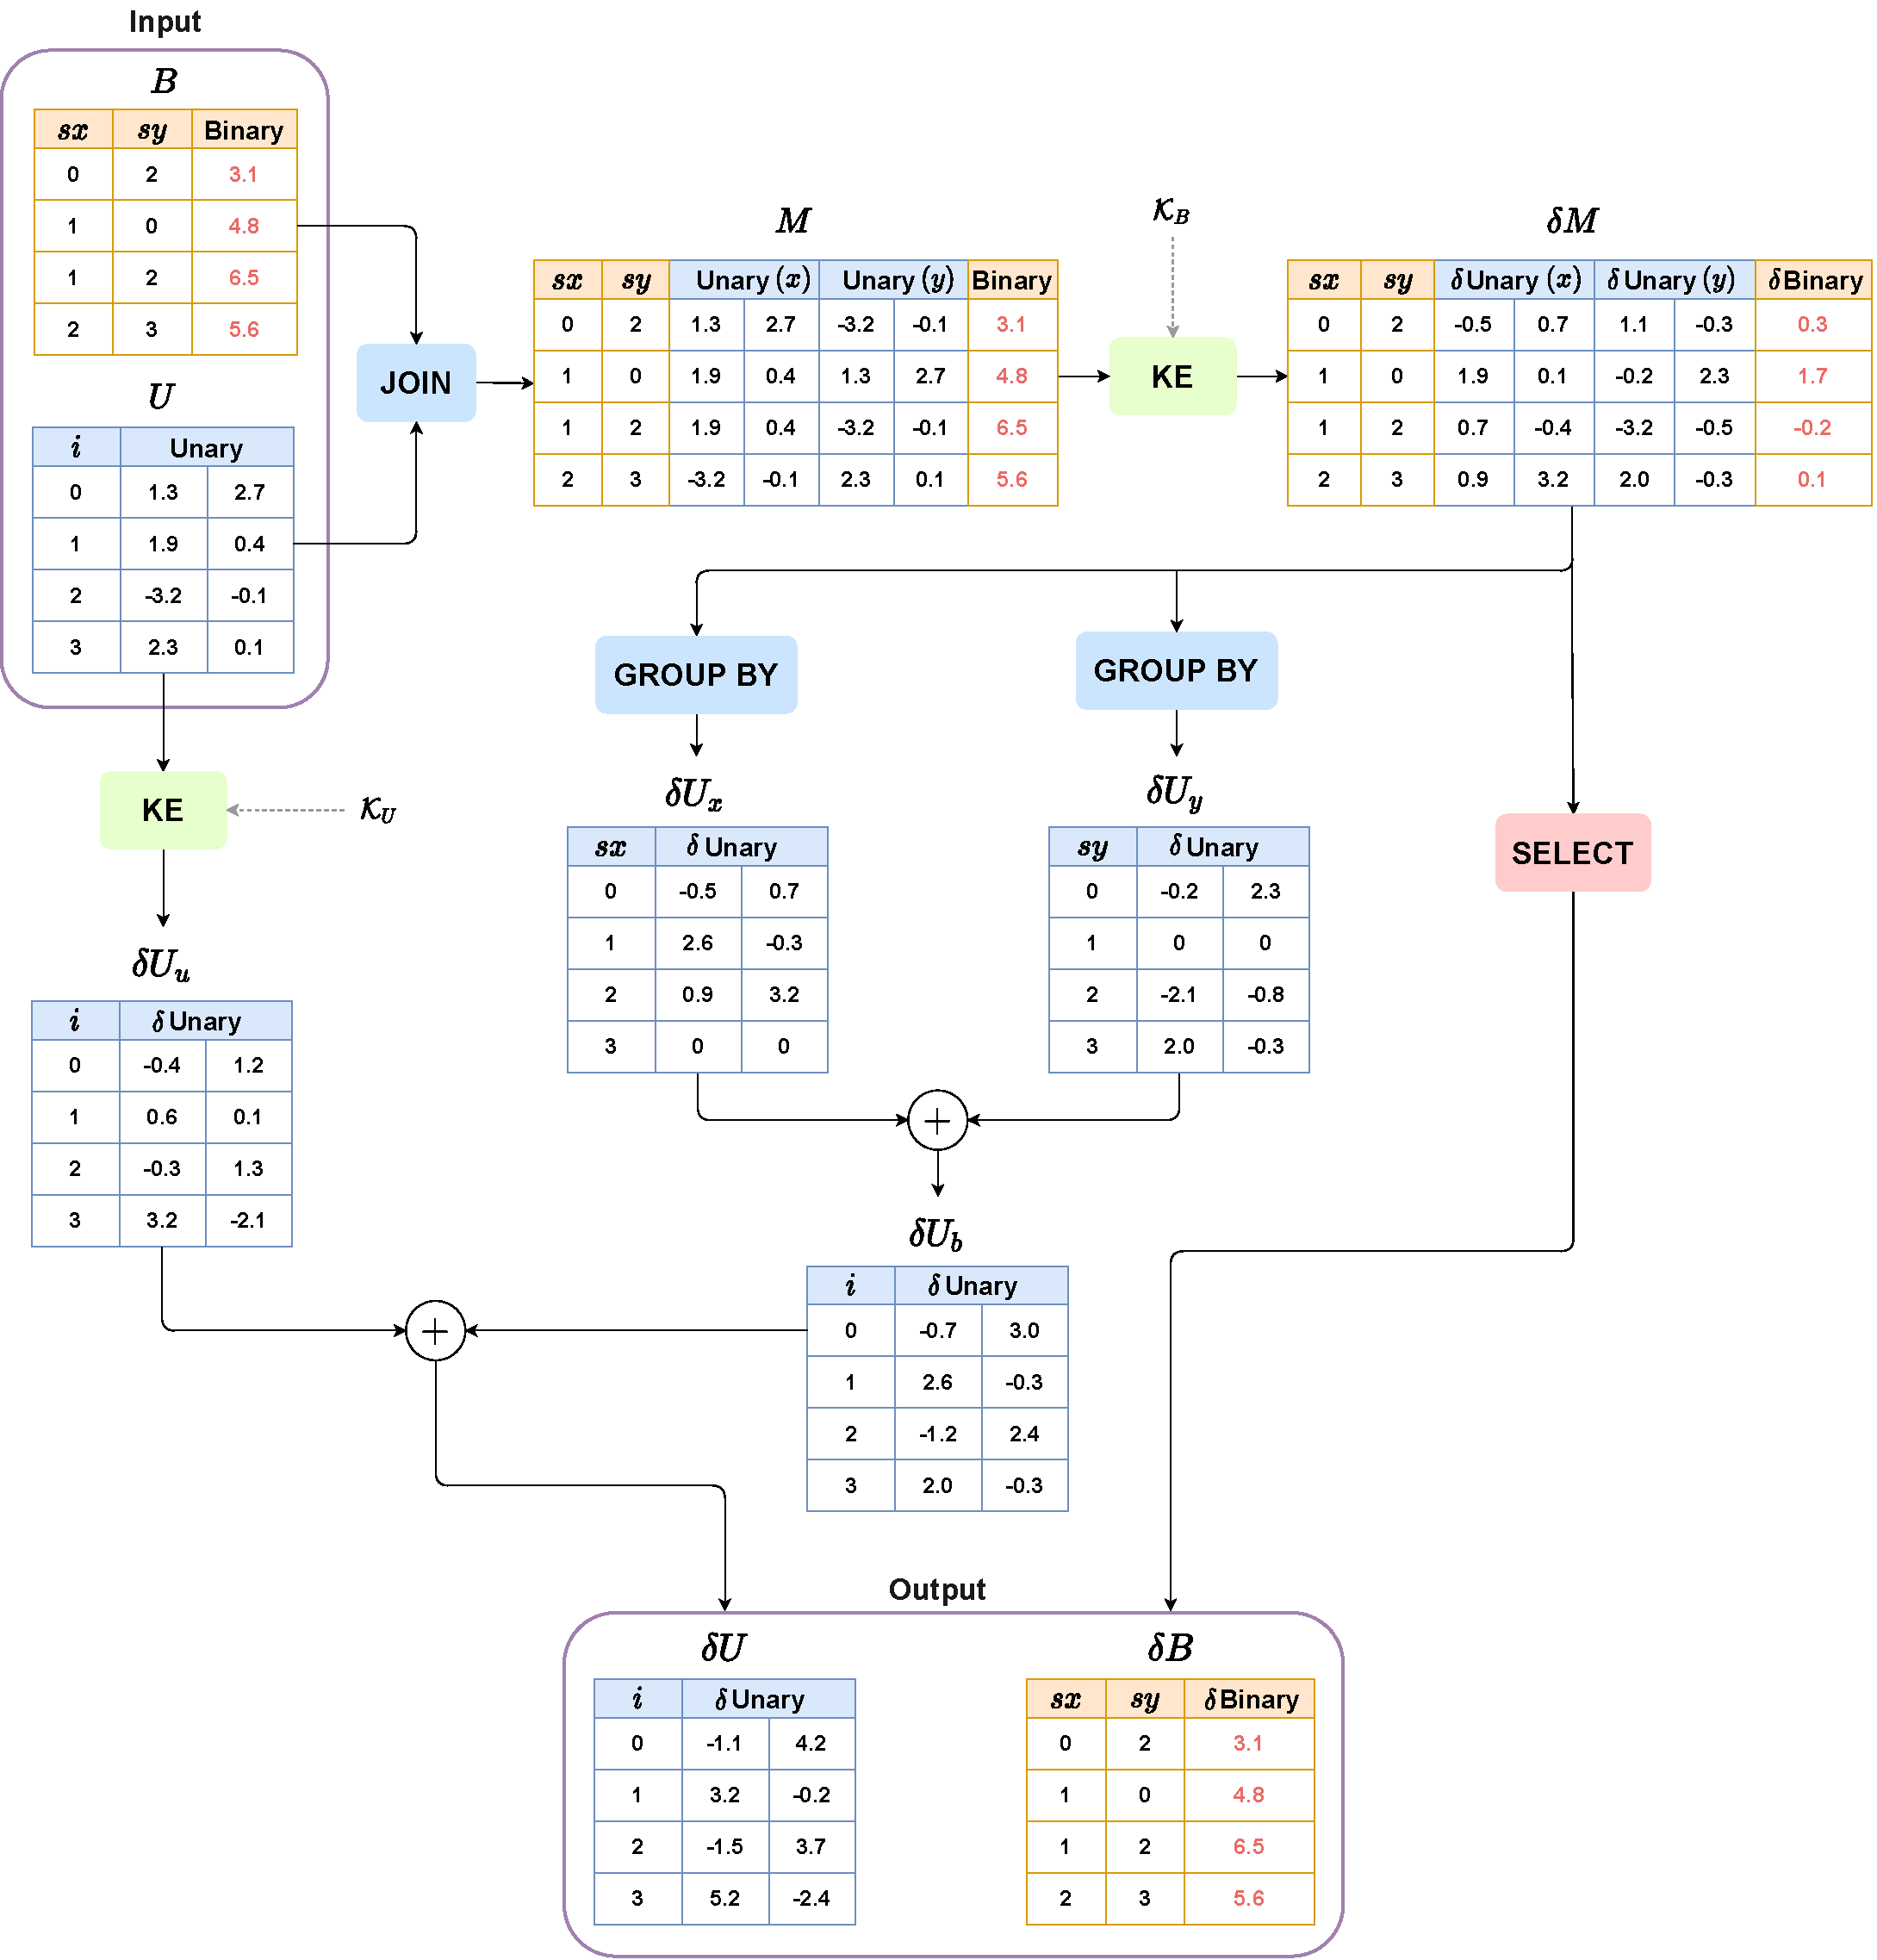
\includegraphics[width=0.65\linewidth]{images/kenn_relational_global_chart.pdf}
	\end{figure}
\end{frame}

\begin{frame}{Appendix: Clause Weights learning}
	\begin{figure}
		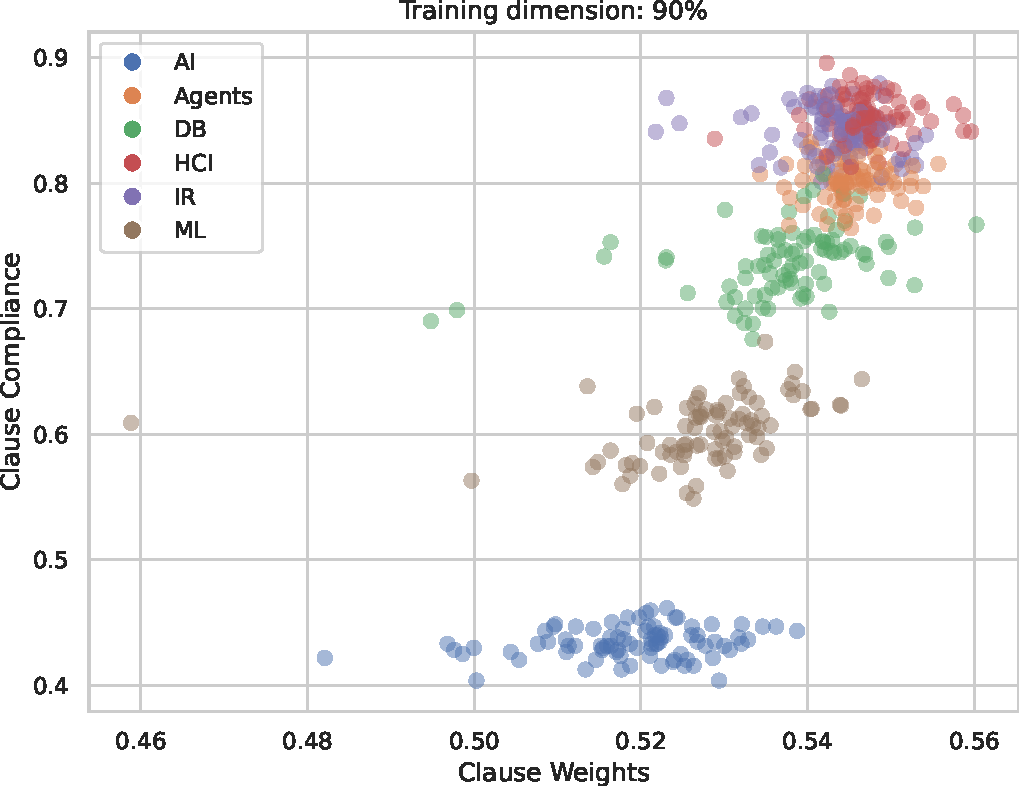
\includegraphics[width=0.75\linewidth]{images/scatter_90.pdf}
	\end{figure}
\end{frame}


\backupend








\end{document}
